\begin{figure}[h!]
	\centering
	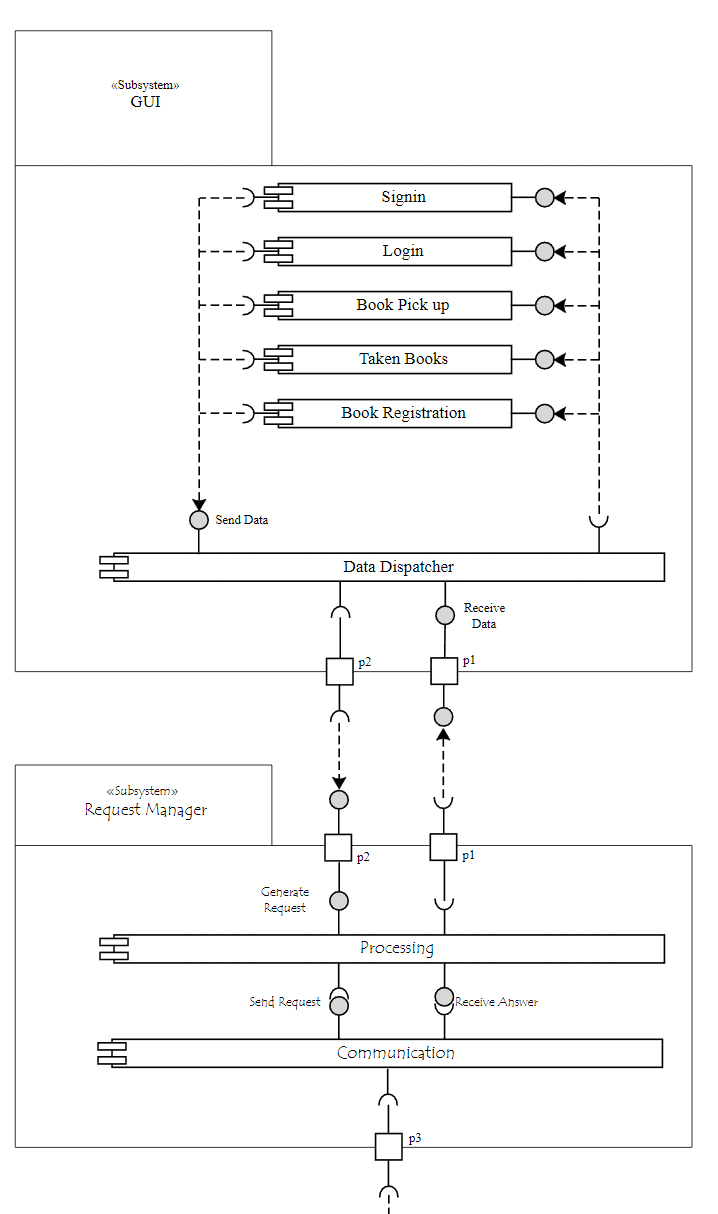
\includegraphics[width=0.8\textwidth]{Immagini/Logical_View_part1}
	\caption{Logical view}
	\label{fig:LogicalView1}
\end{figure}
\begin{figure}[h!]
	\centering
	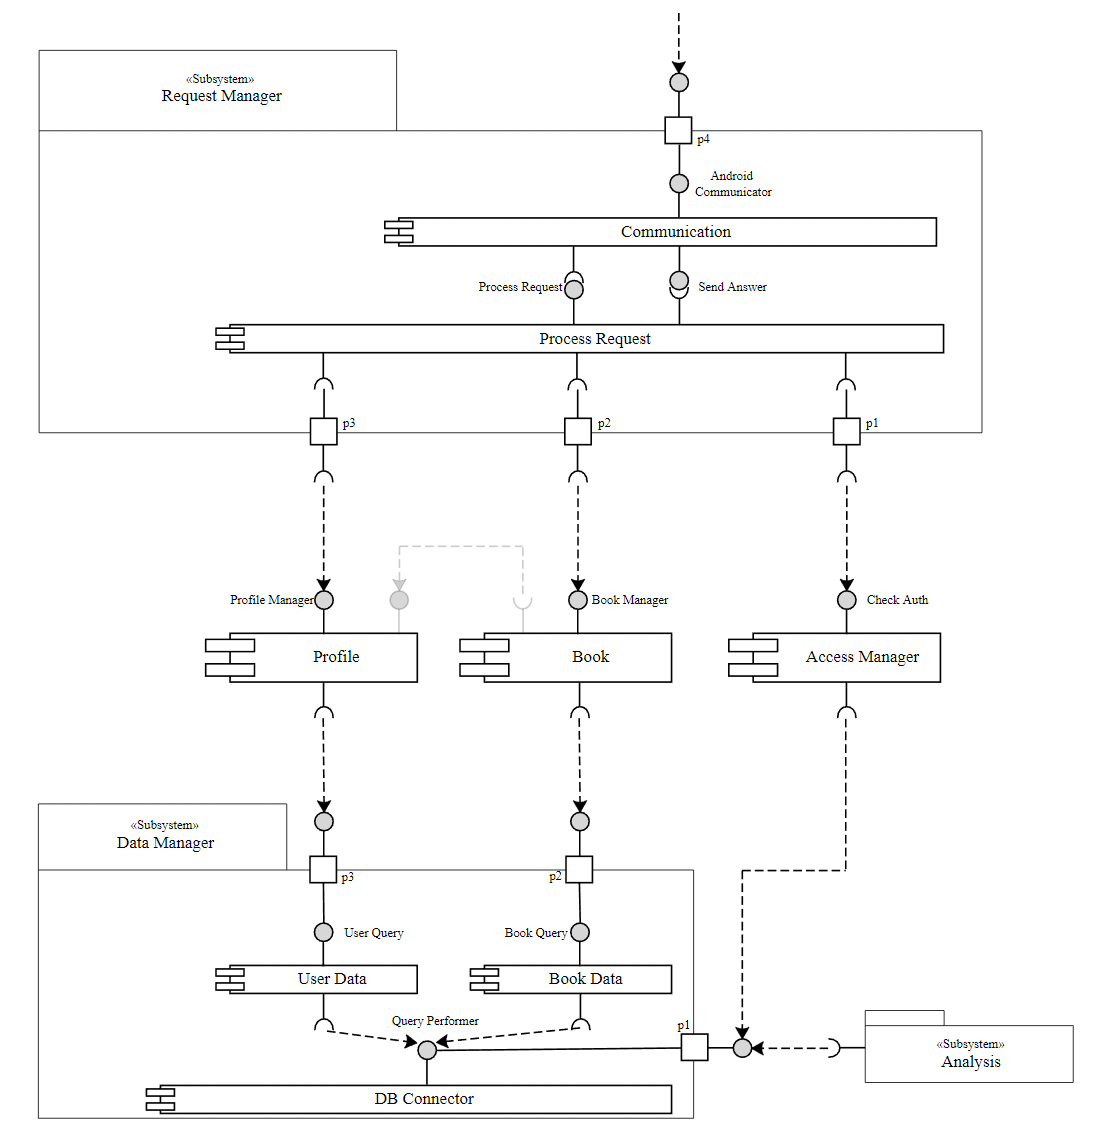
\includegraphics[width=0.8\textwidth]{Immagini/Logical_View_part2}
	\caption{Logical view}
	\label{fig:LogicalView2}
\end{figure}
\noindent
In figura ~\ref{fig:LogicalView1} e ~\ref{fig:LogicalView2} è mostrata la Logical View del sistema progettato. Si può osservare che segue il modello definito attraverso il pattern archietteturale Model View Controller/Presenter, dal momento che vengono individuati tre strati, ciascuno dei quali con le seguenti caratteristiche:
\begin{itemize}
	\item \textbf{Subsystem \textit{"GUI”:}} Rappresenta l’interfaccia grafica con la quale l’applicazione si presenterà. Ciascun componente fa riferimento ad una azione che può essere svolta attraverso lo smartphone, come l’accesso alla rete di Book Crossing(Login) o registrazione di un  libro. Questi componenti saranno quindi allocati direttamente sul dispositivo mobile. 
	\item \textbf{Subsystem \textit{"Request Manager”:}} Ha il compito di gestire le richieste provenienti da ciascun componente descritto nel subsystem \textit{GUI”}. Al suo interno sono indicati i componenti attraverso i quali si risponde alle chiamate provenienti dal client. Questo quindi descrive i componenti che saranno individuati sul server presente all’interno dell’architettura.
	\item \textbf{Subsystem \textit{"Data Manager":}} ”: Rappresenta la comunicazione con il Database. Sono quindi indicati i componenti con i quali il sistema si interfaccerà con la banca dati dell’architettura.
\end{itemize}
Il modello architetturale MVC è stato poi applicato anche successivamente per la progettazione delle componenti previste per ciascun elemento dell'architettura.